\section{Parallélisation du code (MPI) --- Deuxième façon}

\subsection{Stratégie de parallélisation}

\subsubsection{Objectif}

L'objectif de cette étape est d'implémenter la ``deuxième façon'' du sujet :
au lieu de répliquer toute la carte de phéromones sur chaque rang (MPI1), on
répartit la grille par sous-domaines, avec échanges locaux entre voisins.
Le but est de réduire le coût de communication globale et d'améliorer la
scalabilité en fonction du nombre de processus.

\subsubsection{Choix d'architecture}

Dans notre implémentation, le mode \texttt{mpi2} est porté par un backend séparé
\texttt{mpi2+soa}, sélectionné via \texttt{--exec mpi2 --layout soa}.
Les modes \texttt{serial}, \texttt{omp} et \texttt{mpi1} restent inchangés.
Cette séparation permet d'analyser MPI2 sans introduire de régression sur les
modes déjà validés.

\subsubsection{Répartition du travail et données locales}

Nous utilisons une décomposition 1D par lignes :
\begin{itemize}[leftmargin=*]
  \item chaque rang possède un bloc contigu de lignes \(y_0 \dots y_1\),
  \item les voisins MPI sont \texttt{up} et \texttt{down},
  \item chaque rang stocke une carte locale \(V1/V2\) avec halo de 1 cellule.
\end{itemize}

Les fourmis gardent leurs coordonnées globales \((x,y)\), mais ne sont
traitées localement que si leur position appartient au sous-domaine du rang.

\subsubsection{Communications}

MPI2 remplace les réductions globales de carte par des échanges locaux :
\begin{itemize}[leftmargin=*]
  \item \textbf{halo exchange} (\texttt{MPI\_Sendrecv}) pour les lignes frontière
  de \(V1/V2\),
  \item \textbf{migration de fourmis} via buffers agrégés (count + tableau POD)
  entre voisins.
\end{itemize}

Le compteur de nourriture est agrégé avec \texttt{MPI\_Allreduce(SUM)}.
Les temps MPI sont reportés en wall-time via \texttt{MPI\_Allreduce(MAX)}.
La sortie benchmark est root-only (rang 0), comme pour MPI1.

\subsubsection{Politique de migration (baseline)}

Le noyau de déplacement peut faire plusieurs sous-pas par itération
(\texttt{consumed\_time < 1.0}).
Dans la baseline MPI2, nous utilisons une migration différée :
si une fourmi sort du sous-domaine, elle est envoyée au voisin mais ne continue
pas ses sous-pas restants pendant la même itération.
Cette approximation est explicitement documentée pour rester lisible en cadre projet.

\subsection{Résultat du Profilage}

\subsubsection{Protocole expérimental}

Campagne utilisée :
\begin{itemize}[leftmargin=*]
  \item \texttt{results/test\_mpi2\_report\_v1/mpi2/soa/latest}
\end{itemize}

Commande type:
\begin{verbatim}
./scripts/measure_mpi2.sh --folder test_mpi2_report_v1 \
  --np 1,2,4,8 --iterations 400 --warmup 100 --reps 3
\end{verbatim}

Configuration :
\begin{itemize}[leftmargin=*]
  \item 400 itérations, 100 warm-up, donc 300 itérations mesurées,
  \item 3 répétitions par configuration,
  \item \texttt{OMP\_NUM\_THREADS=1}, \texttt{OMP\_DYNAMIC=FALSE},
  \item binding MPI : \texttt{--bind-to core --map-by core},
  \item machine : AMD Ryzen 7 5800H (WSL2).
\end{itemize}

La variation relative du temps noyau est définie par :
\[
\Delta(K0_p)=K0_p-K0_1,
\qquad
\Delta_{\%}(K0_p)=100\times\frac{K0_p-K0_1}{K0_1}
\]
où \(K0_1\) est la valeur à \(np=1\).

\begin{table}[H]
\centering
\scriptsize
\caption{MPI2 SoA : temps noyau, variation relative et speedup selon le nombre de processus}
\label{tab:mpi2-speedup}
\begin{tabular}{@{}rrrrrrr@{}}
\toprule
\textbf{np} & \textbf{K0 moyen} & \textbf{écart-type} & \textbf{\(\Delta\)} & \textbf{\(\Delta_{\%}\)} & \textbf{Speedup \(S(p)\)} & \textbf{Efficacité \(E(p)\)} \\
\midrule
1 & 15.146929 & 0.634749 & +0.000000 & +0.000 & 1.000000 & 1.000000 \\
2 & 8.186620 & 0.534566 & -6.960309 & -45.952 & 1.850205 & 0.925103 \\
4 & 4.656974 & 0.489330 & -10.489955 & -69.255 & 3.252526 & 0.813131 \\
8 & 6.296121 & 1.126444 & -8.850808 & -58.433 & 2.405756 & 0.300719 \\
\bottomrule
\end{tabular}
\end{table}

\[
S_{\text{th,idéal}}(p)=p
\]

\begin{table}[H]
\centering
\caption{Comparaison speedup mesuré vs speedup théorique (MPI2 SoA)}
\label{tab:mpi2-speedup-theory}
\begin{tabular}{@{}rrrr@{}}
\toprule
\textbf{np} & \textbf{\(S_{\text{mesuré}}(p)\)} & \textbf{\(S_{\text{th,idéal}}(p)\)} & \textbf{\(S_{\text{th,Amdahl}}(p)\)} \\
\midrule
1 & 1.000000 & 1.000000 & 1.000000 \\
2 & 1.850205 & 2.000000 & 1.501283 \\
4 & 3.252526 & 4.000000 & 2.003424 \\
8 & 2.405756 & 8.000000 & 2.405756 \\
\bottomrule
\end{tabular}
\end{table}

La comparaison montre que MPI2 reste nettement en-dessous du modèle idéal linéaire,
mais suit une tendance compatible avec une borne d'Amdahl simple (calée sur \(np=8\)).
Cela indique un gain de parallélisme réel, limité à haut \(np\) par les surcoûts de communication.

\subsubsection{Définition et lecture de l'efficacité}

Le speedup est défini par :
\[
S(p)=\frac{T(1)}{T(p)}
\]
et l'efficacité par :
\[
E(p)=\frac{S(p)}{p}
\]

Une efficacité proche de 1 signifie que les processus supplémentaires sont bien
utilisés. Quand \(E(p)\) baisse, cela indique qu'une partie du gain est absorbée
par les overheads (communication, synchronisation, déséquilibre éventuel).
Dans cette campagne, l'efficacité reste élevée à \(np=2\) et \(np=4\), puis chute
nettement à \(np=8\), ce qui indique un changement de régime dominé par la communication.

\begin{table}[H]
\centering
\caption{Décomposition du noyau MPI2 SoA}
\label{tab:mpi2-breakdown}
\begin{tabular}{@{}rrrrrr@{}}
\toprule
\textbf{np} & \textbf{K1} & \textbf{K4} & \textbf{K5} & \(\mathbf{K_{\text{MPI\_sync}}}\) & \(\mathbf{K_{\text{MPI\_halo}}+K_{\text{MPI\_migrate}}}\) \\
\midrule
1 & 12.306339 & 1.623108 & 0.031015 & 0.010476 & 0.004256 \\
2 & 5.985056 & 0.876899 & 0.016374 & 0.862798 & 0.286338 \\
4 & 2.767057 & 0.482712 & 0.012416 & 1.092852 & 0.516112 \\
8 & 1.444341 & 0.323934 & 0.018483 & 2.627381 & 2.602558 \\
\bottomrule
\end{tabular}
\end{table}

\begin{figure}[H]
  \centering
  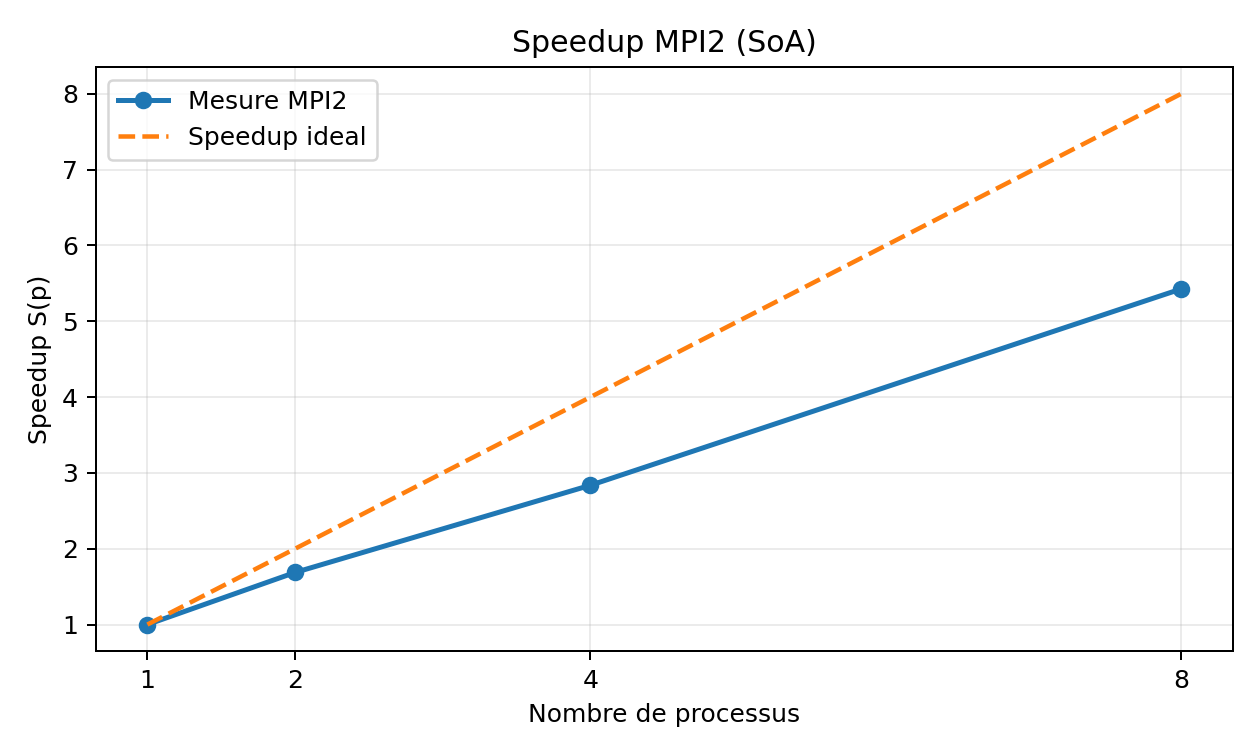
\includegraphics[width=0.82\textwidth]{imgs/mpi2/mpi2_speedup.png}
  \caption{Speedup mesuré MPI2 (SoA) vs speedup idéal linéaire}
  \label{fig:mpi2-speedup}
\end{figure}

\begin{figure}[H]
  \centering
  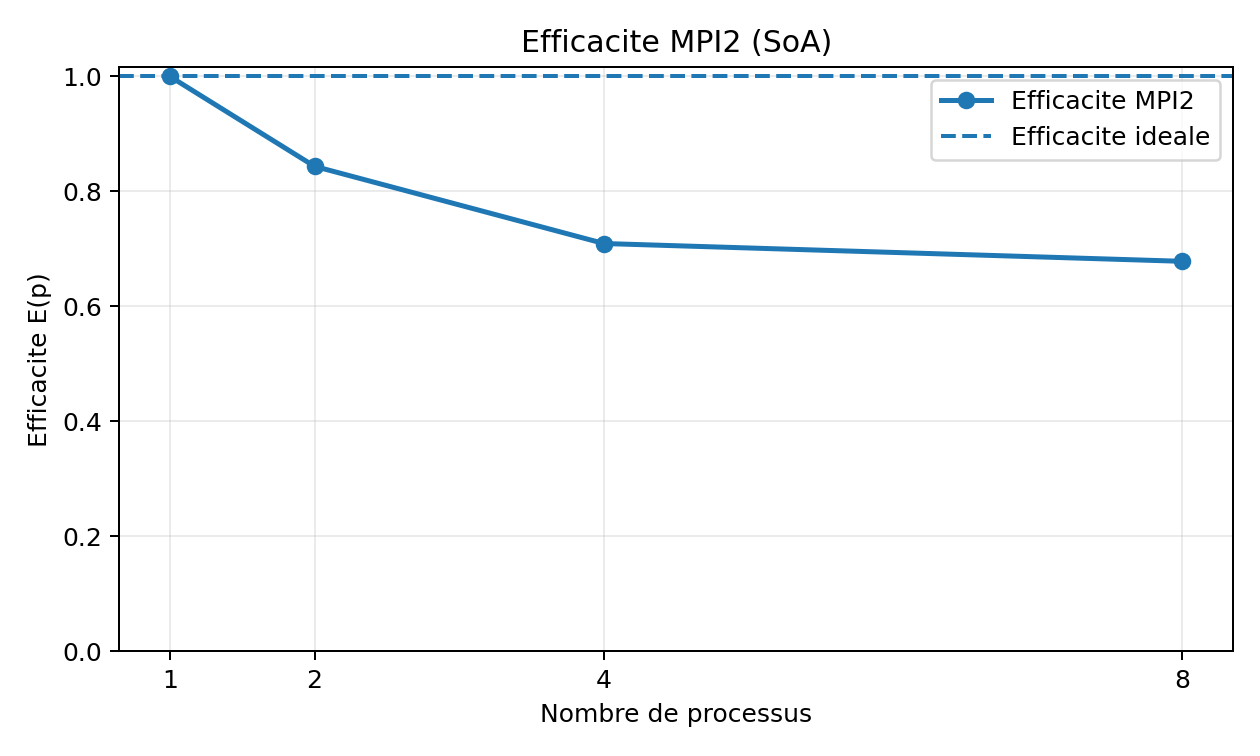
\includegraphics[width=0.82\textwidth]{imgs/mpi2/mpi2_efficiency.png}
  \caption{Efficacité MPI2 (SoA) en fonction du nombre de processus}
  \label{fig:mpi2-efficiency}
\end{figure}

\begin{figure}[H]
  \centering
  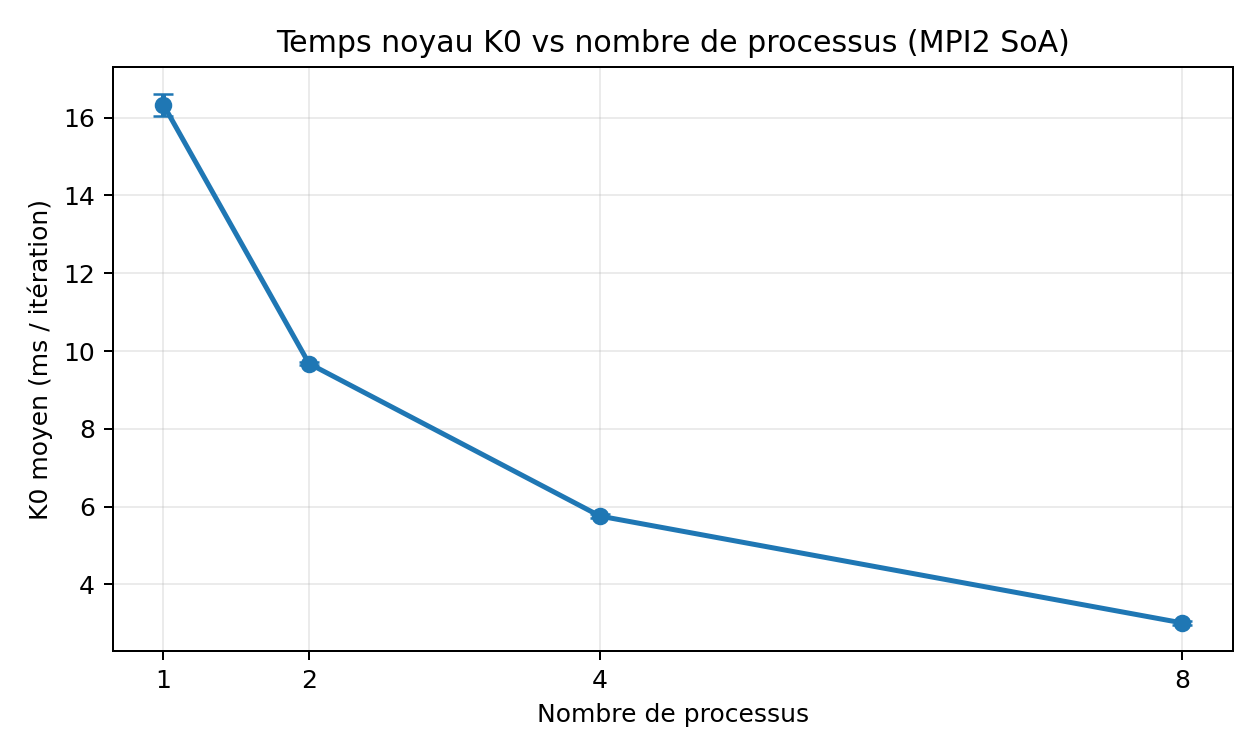
\includegraphics[width=0.82\textwidth]{imgs/mpi2/mpi2_k0_ms_iter.png}
  \caption{Temps noyau \(K0\) en fonction du nombre de processus (MPI2 SoA)}
  \label{fig:mpi2-k0}
\end{figure}

\begin{figure}[H]
  \centering
  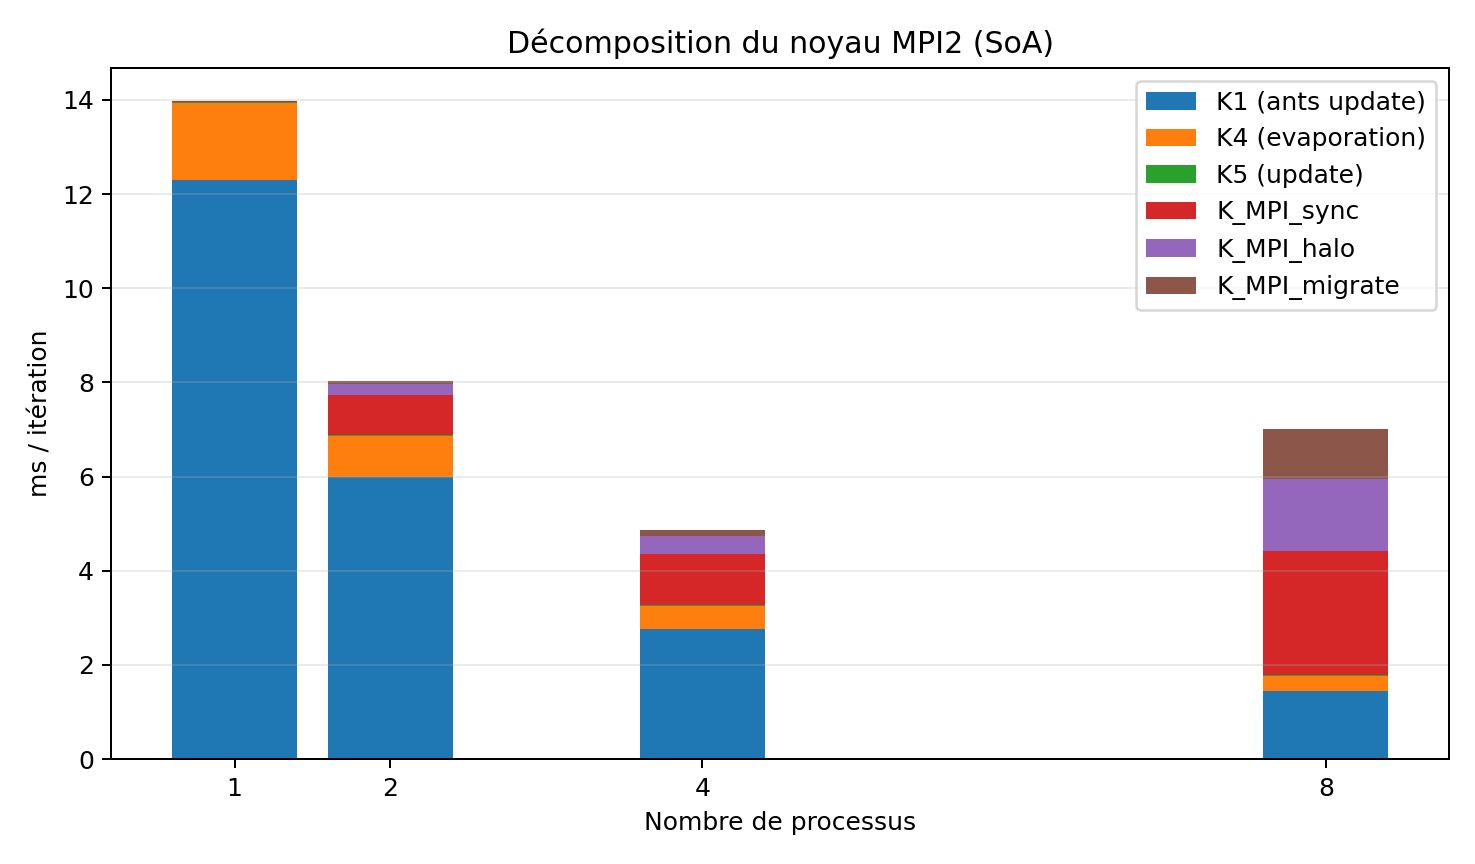
\includegraphics[width=0.84\textwidth]{imgs/mpi2/mpi2_kernel_breakdown.png}
  \caption{Décomposition \(K1/K4/K5/K_{\text{MPI\_sync}}/K_{\text{MPI\_halo}}/K_{\text{MPI\_migrate}}\)}
  \label{fig:mpi2-breakdown}
\end{figure}

\subsection{Analyse des Résultats}

\subsubsection{Scalabilité globale}

Les résultats montrent une amélioration nette de \(K0\) quand \(np\) augmente
(Table~\ref{tab:mpi2-speedup}) jusqu'à \(np=4\) :
\[
S(2)=1.850,\quad S(4)=3.253,\quad S(8)=2.406
\]
Le speedup reste sous la droite idéale, et on observe une régression à \(np=8\)
par rapport à \(np=4\), signe d'un coût de communication dominant à haut \(np\).

La Table~\ref{tab:mpi2-speedup-theory} permet de lire directement cet écart:
à \(np=4\), MPI2 reste relativement proche de l'idéal (\(3.25\) vs \(4.00\)),
alors qu'à \(np=8\), la distance devient forte (\(2.41\) vs \(8.00\)).

\subsubsection{Lecture Amdahl}

Avec \(S(8)=2.406\), une estimation simple donne :
\[
f \approx \frac{8/S(8)-1}{7}\approx 0.332,\qquad
S_{\max}\approx \frac{1}{f}\approx 3.01
\]
Cette lecture est cohérente avec les mesures: à \(np=8\), la part non-calcul
(synchronisation + échanges) devient majoritaire.

\subsubsection{Bottlenecks observés}

La Table~\ref{tab:mpi2-breakdown} montre que :
\begin{itemize}[leftmargin=*]
  \item \(K1\) diminue bien avec \(np\) (travail fourmis distribué),
  \item \(K_{\text{MPI\_sync}}\) et \(K_{\text{MPI\_halo}}+K_{\text{MPI\_migrate}}\) augmentent
  nettement à partir de \(np=4\),
  \item à \(np=8\), les coûts de communication cumulés (\(\approx 5.23\) ms/it) deviennent
  du même ordre que \(K0\), ce qui limite fortement la scalabilité.
\end{itemize}

En pratique, MPI2 évite bien les réductions globales de cartes complètes (cas MPI1), mais
le coût des échanges locaux (halo + migration) devient dominant quand le nombre de processus
augmente trop pour cette taille de problème.

\subsubsection{Lecture de l'efficacité}

La Figure~\ref{fig:mpi2-efficiency} confirme la baisse de l'efficacité quand \(np\) augmente :
\[
E(2)=0.925,\quad E(4)=0.813,\quad E(8)=0.301
\]
L'efficacité reste bonne jusqu'à \(np=4\), puis chute à \(np=8\), ce qui est cohérent
avec une surcharge de communication et de synchronisation.

\subsection{Interprétation}

Les Tables~\ref{tab:mpi2-speedup} et \ref{tab:mpi2-breakdown}, ainsi que les Figures
~\ref{fig:mpi2-speedup}, \ref{fig:mpi2-efficiency}, \ref{fig:mpi2-k0} et \ref{fig:mpi2-breakdown},
montrent que la ``deuxième façon'' atteint l'objectif principal du point MPI :
réduire la communication globale par rapport à MPI1, avec un gain net jusqu'à \(np=4\).

Le point important est que cette amélioration ne vient pas d'une optimisation locale isolée,
mais d'un changement de stratégie de communication :
au lieu de synchroniser des cartes complètes par \texttt{Allreduce(MAX)} à chaque itération,
on échange principalement des informations de bord (halo) et des fourmis migrantes entre voisins.

Dans cette nouvelle campagne, on voit cependant la limite de granularité :
pour \(np=8\), le coût des échanges locaux devient trop élevé par rapport au calcul local,
ce qui fait baisser speedup et efficacité.

\subsection{Proposition de réponse à la question bonus}

Pour répondre à la question bonus, nous proposerions d'aller un pas plus loin que la
simple description de stratégie : l'idée serait de mettre réellement en oeuvre MPI2,
puis de mesurer l'accélération obtenue en fonction du nombre de processus.
Le but ne serait donc pas seulement de ``faire une version MPI'', mais de vérifier si
la décomposition de domaine permet bien de réduire le coût de communication par rapport
à MPI1.

La stratégie retenue resterait celle décrite dans cette section :
une décomposition 1D par lignes, un halo de 1 cellule pour lire correctement les voisins,
et une migration des fourmis uniquement entre processus adjacents.
De manière intuitive, chaque rang travaillerait sur sa propre zone de la carte
et n'échangerait que ce qui est nécessaire avec ses voisins, au lieu de resynchroniser
la carte complète à chaque itération.
Cette approche suit directement les idées du cours :
\emph{domain decomposition}, communications locales, et réduction du volume de données échangées.

L'idée serait ensuite de mesurer le temps noyau \(K0\) pour plusieurs valeurs de \(np\),
par exemple \(np \in \{1,2,4,8\}\), en gardant exactement la même configuration globale
(même nombre total de fourmis, même taille de carte, un coeur par processus).
L'accélération pourrait alors être calculée par :
\[
S(p)=\frac{T(1)}{T(p)}
\qquad\text{et}\qquad
E(p)=\frac{S(p)}{p}
\]
où \(T(1)\) serait le temps du backend \texttt{mpi2+soa} avec un seul processus,
et \(T(p)\) le temps du même backend avec \(p\) processus.
Ce choix de référence permettrait d'évaluer l'effet du parallélisme MPI sans mélanger
les différences algorithmiques avec les versions \texttt{serial} ou \texttt{omp}.

Pour rendre l'analyse lisible, nous proposerions de reporter au minimum un tableau
avec \(np\), \(K0\), \(S(p)\) et \(E(p)\), ainsi qu'une décomposition plus fine
de \(K1\), \(K4\), \(K5\), \(K_{\text{MPI\_halo}}\) et \(K_{\text{MPI\_migrate}}\).
Ainsi, on pourrait voir non seulement si MPI2 accélère, mais aussi à partir de quel point
les échanges de halo et la migration des fourmis commencent à limiter le gain.

De façon intuitive, on s'attendrait à ce que le temps baisse d'abord quand \(np\) augmente,
car chaque processus traite moins de calcul local.
En revanche, quand \(np\) devient trop grand par rapport à la taille du problème,
le coût des communications locales et le déséquilibre de charge peuvent prendre le dessus.
On s'attendrait donc à observer un speedup réel mais non linéaire, avec une efficacité
qui baisse progressivement lorsque le nombre de processus devient trop élevé.

En conclusion, cette réponse au bonus consisterait à montrer que la stratégie MPI2 est
pertinente pour réduire le coût des synchronisations globales de MPI1, mais que son intérêt
reste conditionné par l'équilibre entre calcul local et communications.
Autrement dit, si MPI2 est bien implémenté, il devrait devenir plus intéressant que MPI1
dès que le coût des \texttt{Allreduce} globaux devient dominant, tout en restant limité
par les échanges de halo, la migration et le \emph{load balancing}.
